\documentclass{article}

% Packages for setting up page margins
\usepackage[margin=1in]{geometry}

\usepackage{graphicx, setspace, amsmath, mathtools, amssymb, url, float}
\setlength{\parskip}{2mm}
\graphicspath{ {./images/} }

% Title
\title{CS451 Introduction to Parallel and Distributed Computing - Assignment 3}
\author{Batkhishig Dulamsurankhor - A20543498}
\date{\today} % Use \date{} for no date

\begin{document}

\maketitle

\begin{enumerate}
  \item Screen shots of your working cluster by taking screen shots at 16,17 and 20. If your cluster isn't working, those commands will fail
  \begin{figure}[H]
    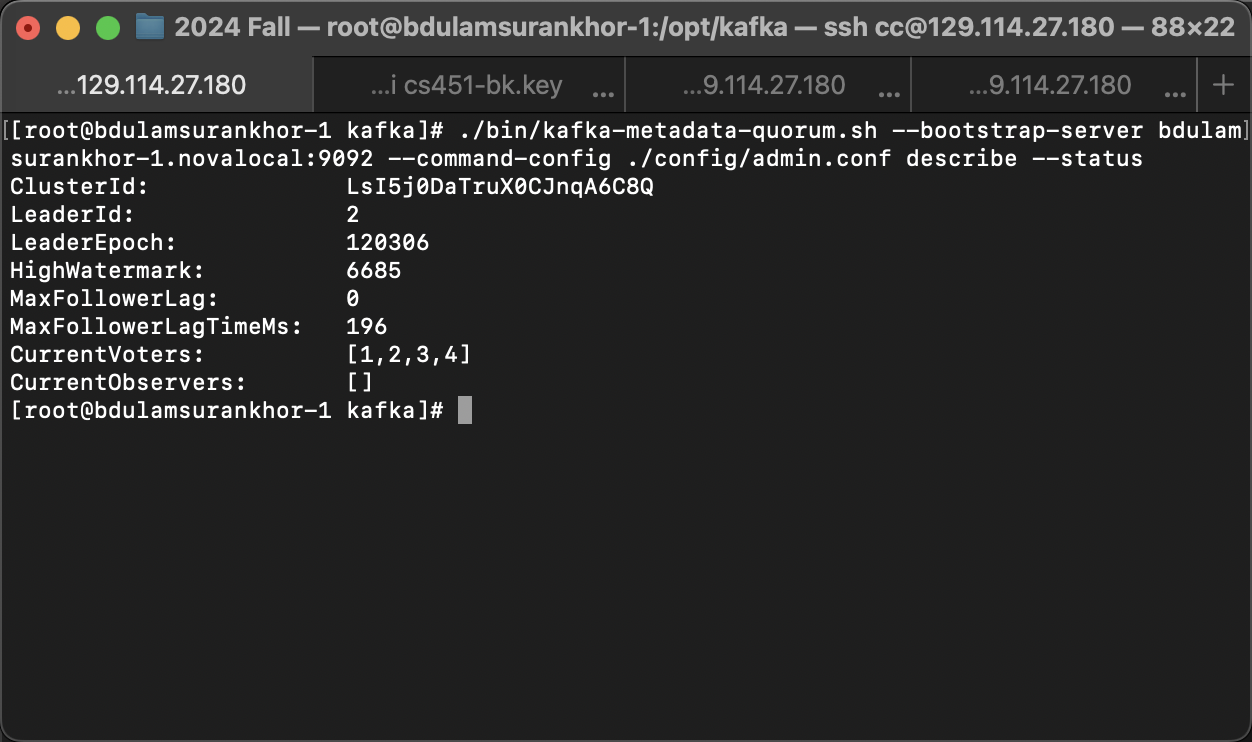
\includegraphics[width=\textwidth]{image1.png}
    \caption{Screenshot at 16.}
    \centering
  \end{figure}
  \begin{figure}[H]
    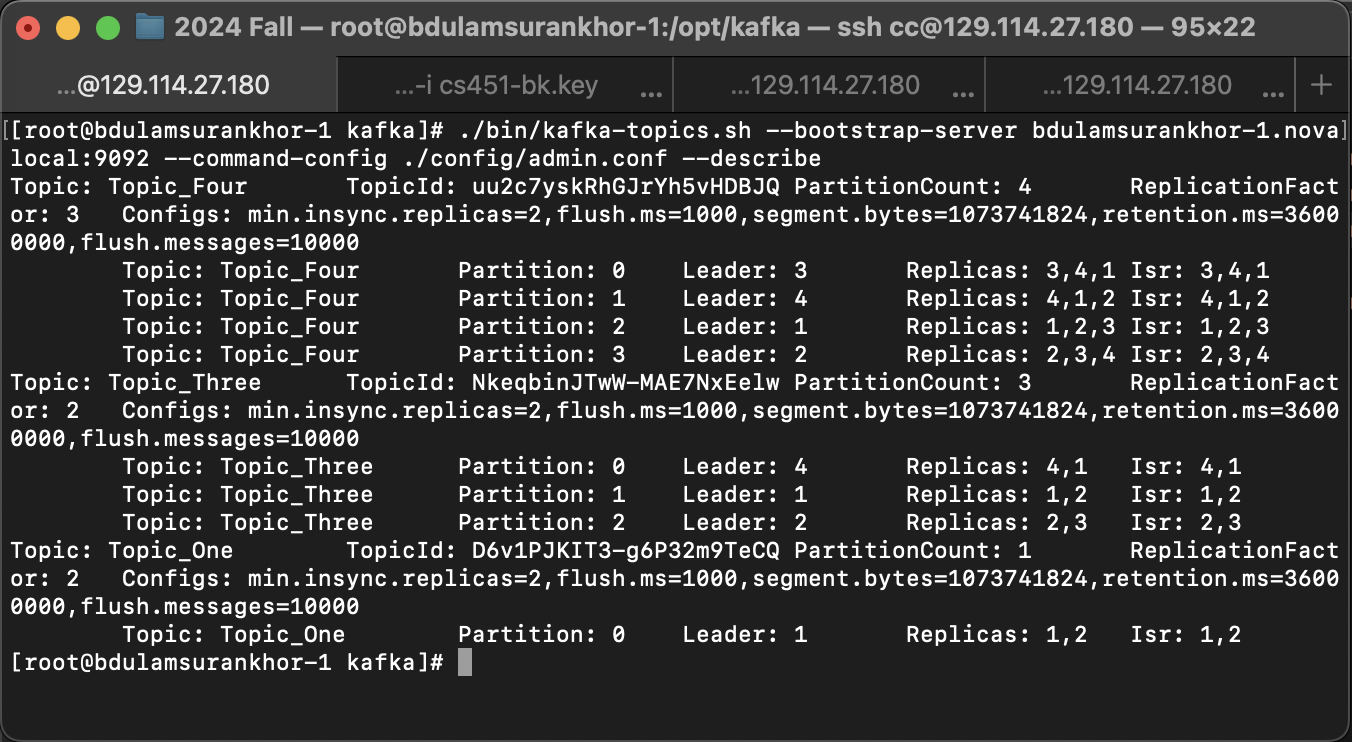
\includegraphics[width=\textwidth]{image2.png}
    \caption{Screenshot at 17.}
    \centering
  \end{figure}
  \begin{figure}[H]
    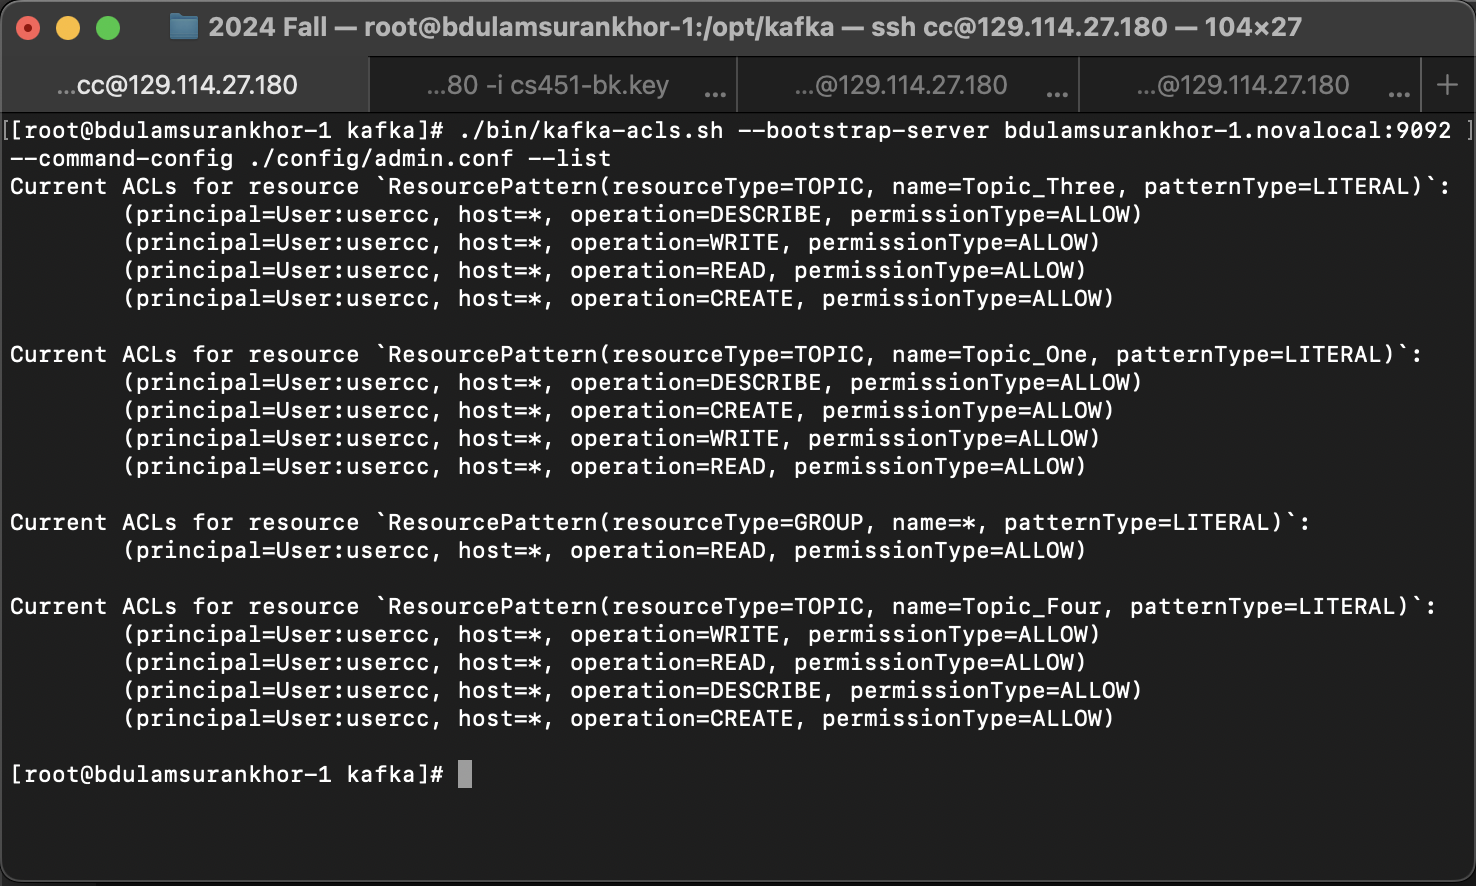
\includegraphics[width=\textwidth]{image3.png}
    \caption{Screenshot at 20.}
    \centering
  \end{figure}
  \item Explain the write process when the producer wrote a message
  \item Why did we enable SSL?
  \item Who and what is the principle?
  \item Shutdown 1 of the 4 nodes, try reading and writing messages like in part 2. What happened to which topic? (sudo systemctl stop kafka)
  \item Shutdown 2 of the 4 nodes, try reading and writing messages like in part 2. What happened to which topic? (sudo systemctl stop kafka)
  \item Start the two back up (sudo systemctl start kafka) on both
  \item Rerun 17.d, are the partitions insync? Take a screenshot
  \item Why is kafka running as the user kafka and not root?
\end{enumerate}

\end{document}